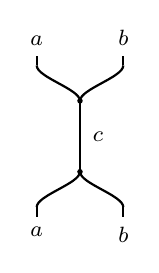
\begin{tikzpicture}[thick, >=stealth, baseline={(current bounding box.center)}, scale=1.000]
\begin{scope}[shift={(0.000,0.000)}, scale=1.000]
  \draw (0.000,0.000) .. controls (0.000,0.300) and (0.000,0.600) .. (0.000,0.900);
  \draw (-0.550,-0.450) .. controls (-0.550,-0.490) and (-0.550,-0.530) .. (-0.550,-0.570);
  \draw (0.550,-0.450) .. controls (0.550,-0.490) and (0.550,-0.530) .. (0.550,-0.570);
  \draw (-0.550,1.350) .. controls (-0.550,1.390) and (-0.550,1.430) .. (-0.550,1.470);
  \draw (0.550,1.350) .. controls (0.550,1.390) and (0.550,1.430) .. (0.550,1.470);
  \draw (0.000,0.000) .. controls (0.000,-0.150) and (-0.550,-0.300) .. (-0.550,-0.450);
  \draw (0.000,0.000) .. controls (0.000,-0.150) and (0.550,-0.300) .. (0.550,-0.450);
  \draw (0.000,0.900) .. controls (0.000,1.050) and (-0.550,1.200) .. (-0.550,1.350);
  \draw (0.000,0.900) .. controls (0.000,1.050) and (0.550,1.200) .. (0.550,1.350);
\end{scope}
\begin{scope}[shift={(0.000,0.000)}, scale=1.000]
  \fill (0.000,0.000) circle (0.035);
  \fill (0.000,0.900) circle (0.035);
\end{scope}
\begin{scope}[shift={(0.000,0.000)}, scale=1.000, every node/.style={inner sep=1pt, font=\footnotesize}]
  \node[anchor=west, fill=white, inner sep=0.8pt] at (0.120,0.450) {$c$};
  \node[anchor=north] at (-0.550,-0.650) {$a$};
  \node[anchor=north] at (0.550,-0.650) {$b$};
  \node[anchor=south] at (-0.550,1.550) {$a$};
  \node[anchor=south] at (0.550,1.550) {$b$};
\end{scope}
\end{tikzpicture}
